% begin module polar-curve-ex8

%plots a section of the second graph:
\newcommand{\plotSection}[1]{%
\psplot[linecolor=red, plotpoints=200]{#1\space 1 sub 6.283185 mul 8 div}{#1\space  6.283185 mul 8 div}{cos(2*x)}%
\fcFullDot{#1\space  1 sub 6.283185 mul 8 div} {#1\space  1 sub 6.283185 mul 8 div 57.29578 mul 2 mul cos }%
\fcFullDot{#1\space  6.283185 mul 8 div} {#1\space  6.283185 mul 8 div 57.29578 mul 2 mul cos }%
}

\begin{frame}
\begin{example} %[Example 8, p. 679]
Sketch the curve $r = \cos (2\theta)$.
\begin{columns}[c]
\column{.3\textwidth}
\psset{xunit=1cm, yunit=1cm,algebraic=true}
\begin{pspicture}(-1.4, -1.6)(1.6,1.6)
\tiny%
\fcAxesStandard{-1.3}{-1.3}{1.6}{1.6}%
\fcLabelXOne%
\fcLabelYOne%
\uncover<2>{%
\fcDrawPolar[linecolor=red, plotpoints=200, arrows=->]{3.141592654 0 mul 4 div}{3.141592654 1 mul 4 div}{cos(2*t)}%
}%
\uncover<3->{%
\fcDrawPolar[linecolor=blue, plotpoints=200]{3.141592654 0 mul 4 div}{3.141592654 1 mul 4 div}{cos(2*t)}%
}%
\uncover<3>{%
\fcDrawPolar[linecolor=red, plotpoints=200, arrows=->]{3.141592654 1 mul 4 div}{3.141592654 2 mul 4 div}{cos(2*t)}%
}%
\uncover<4->{%
\fcDrawPolar[linecolor=blue, plotpoints=200]{3.141592654 1 mul 4 div}{3.141592654 2 mul 4 div}{cos(2*t)}%
}%
\uncover<4>{%
\fcDrawPolar[linecolor=red, plotpoints=200, arrows=->]{3.141592654 2 mul 4 div}{3.141592654 3 mul 4 div}{cos(2*t)}%
}%
\uncover<5->{%
\fcDrawPolar[linecolor=blue, plotpoints=200]{3.141592654 2 mul 4 div}{3.141592654 3 mul 4 div}{cos(2*t)}%
}%
\uncover<5>{%
\fcDrawPolar[linecolor=red, plotpoints=200, arrows=->]{3.141592654 3 mul 4 div}{3.141592654 4 mul 4 div}{cos(2*t)}%
}%
\uncover<6->{%
\fcDrawPolar[linecolor=blue, plotpoints=200]{3.141592654 3 mul 4 div}{3.141592654 4 mul 4 div}{cos(2*t)}%
}%
\uncover<6>{%
\fcDrawPolar[linecolor=red, plotpoints=200, arrows=->]{3.141592654 4 mul 4 div}{3.141592654 5 mul 4 div}{cos(2*t)}%
}%
\uncover<7->{%
\fcDrawPolar[linecolor=blue, plotpoints=200]{3.141592654 4 mul 4 div}{3.141592654 5 mul 4 div}{cos(2*t)}%
}%
\uncover<7>{%
\fcDrawPolar[linecolor=red, plotpoints=200, arrows=->]{3.141592654 5 mul 4 div}{3.141592654 6 mul 4 div}{cos(2*t)}%
}%
\uncover<8->{%
\fcDrawPolar[linecolor=blue, plotpoints=200]{3.141592654 5 mul 4 div}{3.141592654 6 mul 4 div}{cos(2*t)}%
}%
\uncover<8>{%
\fcDrawPolar[linecolor=red, plotpoints=200, arrows=->]{3.141592654 6 mul 4 div}{3.141592654 7 mul 4 div}{cos(2*t)}%
}%
\uncover<9->{%
\fcDrawPolar[linecolor=blue, plotpoints=200]{3.141592654 6 mul 4 div}{3.141592654 7 mul 4 div}{cos(2*t)}%
}%
\uncover<9>{%
\fcDrawPolar[linecolor=red, plotpoints=200, arrows=->]{3.141592654 7 mul 4 div}{3.141592654 8 mul 4 div}{cos(2*t)}%
}%
\uncover<10->{%
\fcDrawPolar[linecolor=blue, plotpoints=200]{3.141592654 7 mul 4 div}{3.141592654 8 mul 4 div}{cos(2*t)}%
}%
\end{pspicture}

%\ \only<handout:0| 1>{%
%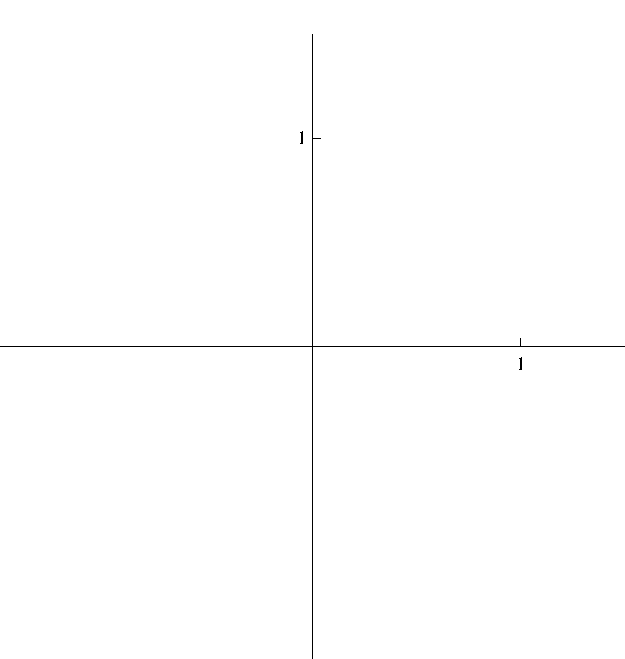
\includegraphics[height=3.6cm]{polar-curves/pictures/11-03-ex8a.pdf}%
%}%
%\only<handout:0| 2>{%
%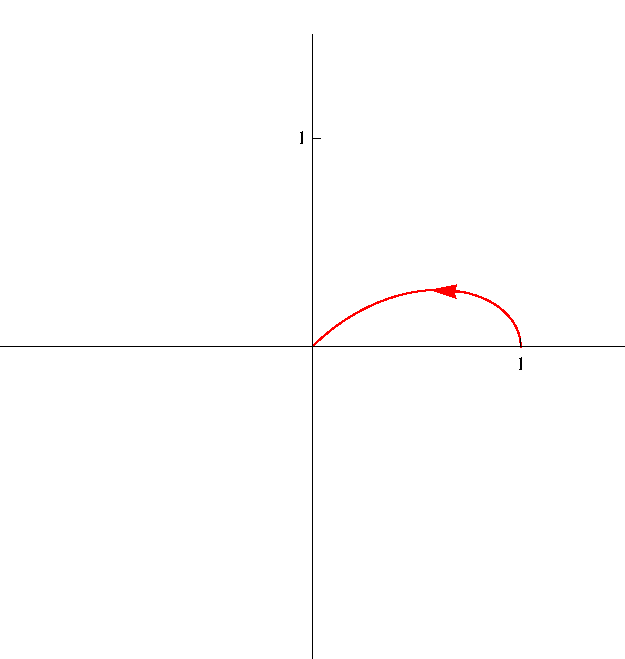
\includegraphics[height=3.6cm]{polar-curves/pictures/11-03-ex8b.pdf}%
%}%
%\only<handout:0| 3>{%
%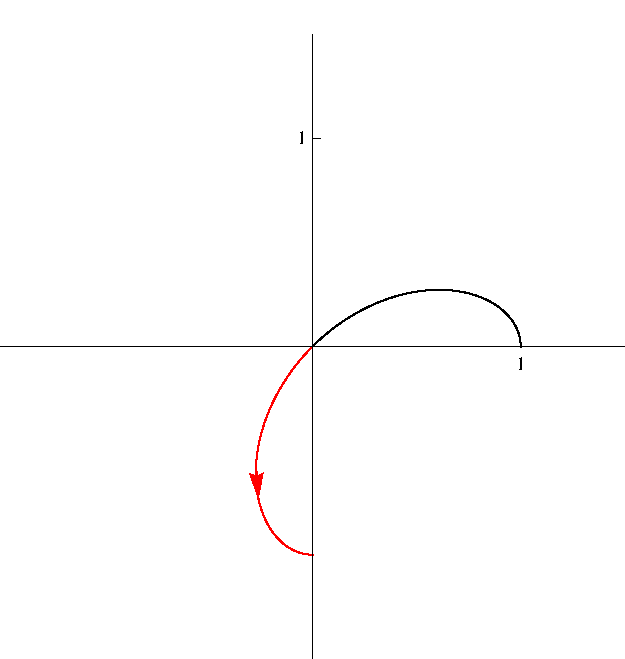
\includegraphics[height=3.6cm]{polar-curves/pictures/11-03-ex8c.pdf}%
%}%
%\only<handout:0| 4>{%
%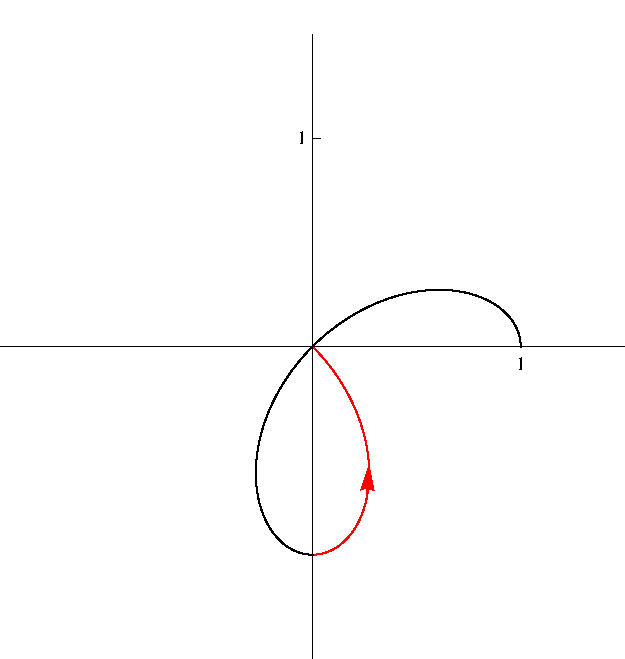
\includegraphics[height=3.6cm]{polar-curves/pictures/11-03-ex8d.pdf}%
%}%
%\only<handout:0| 5>{%
%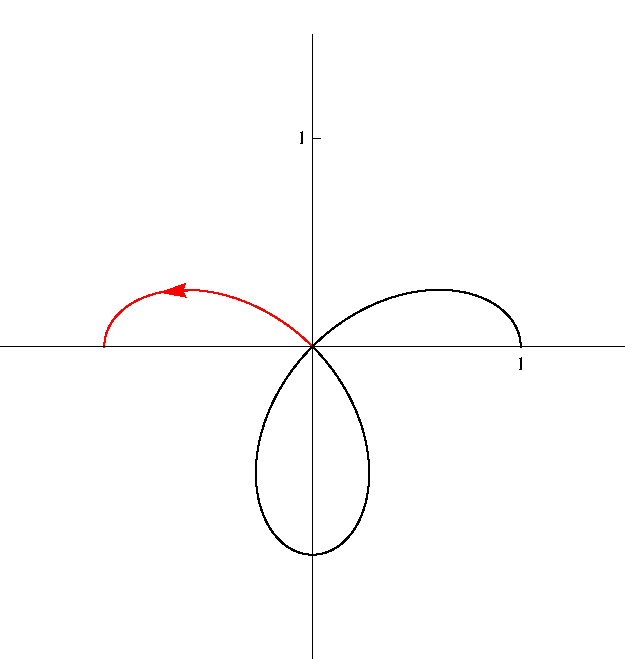
\includegraphics[height=3.6cm]{polar-curves/pictures/11-03-ex8e.pdf}%
%}%
%\only<handout:0| 6>{%
%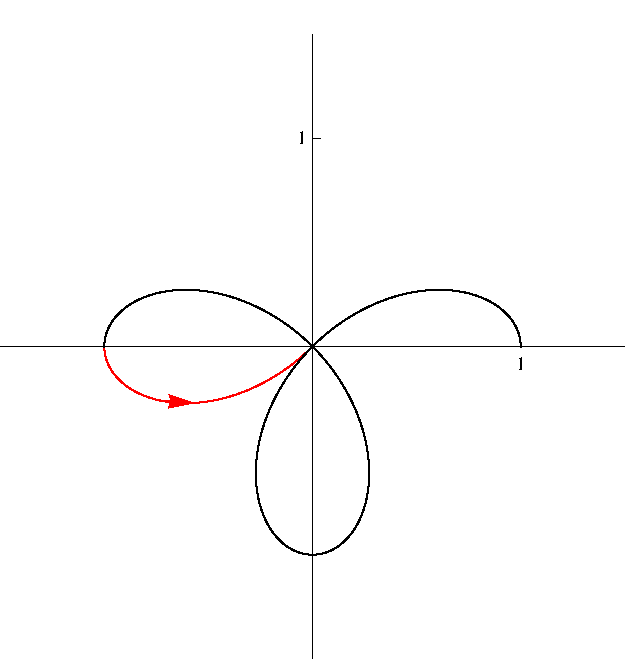
\includegraphics[height=3.6cm]{polar-curves/pictures/11-03-ex8f.pdf}%
%}%
%\only<handout:0| 7>{%
%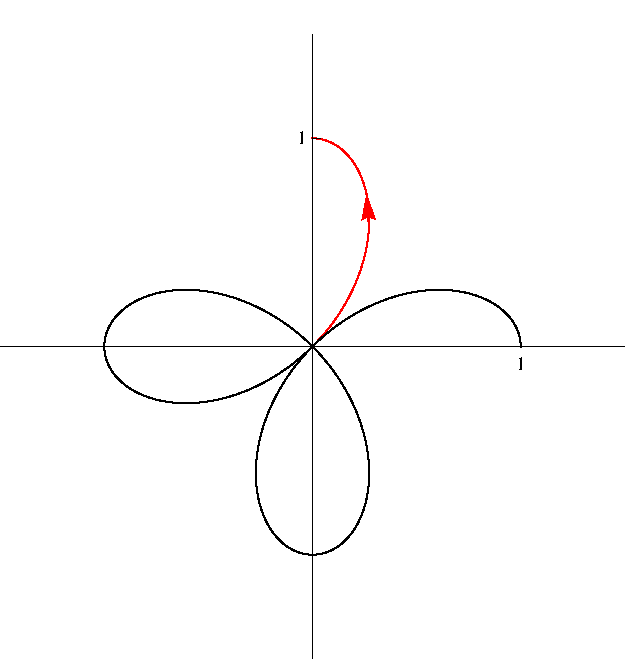
\includegraphics[height=3.6cm]{polar-curves/pictures/11-03-ex8g.pdf}%
%}%
%\only<handout:0| 8>{%
%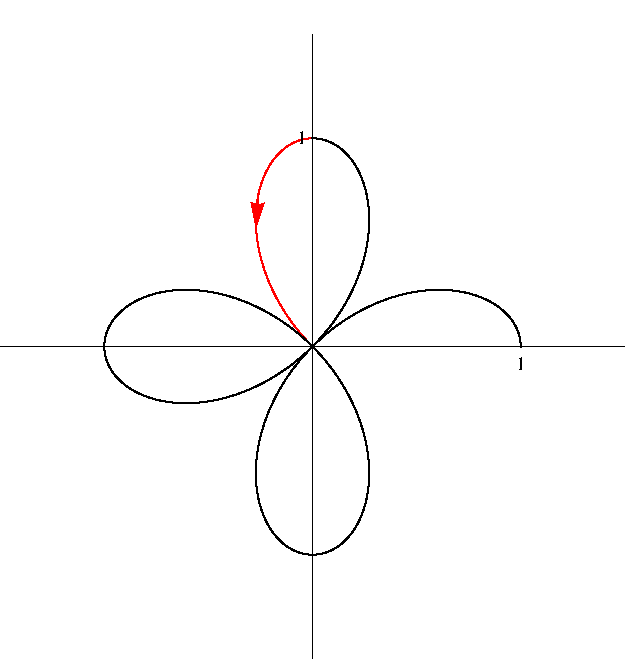
\includegraphics[height=3.6cm]{polar-curves/pictures/11-03-ex8h.pdf}%
%}%
%\only<9->{%
%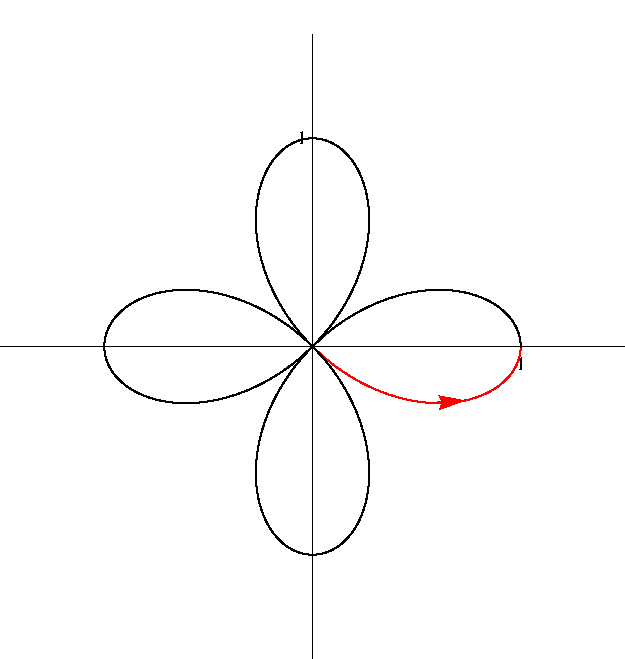
\includegraphics[height=3.6cm]{polar-curves/pictures/11-03-ex8i.pdf}%
%}%
\column{.7\textwidth}
\psset{xunit=1cm, yunit=1cm, algebraic=true}
\begin{pspicture}(-0.7, -1.6)(6.55,1.6)

\tiny
\psframe*[linecolor=white](-0.7, -1.6)(6.55, 1.6)
\psaxes[arrows=<->, Dx=0.785398163, Dy=1, labels=none](0,0)(-0.5, -1.4)(6.4, 1.4)
\rput[r](-0.1,1.4){$r$}
\rput[t](6.48,-0.01){$\theta$}
\rput[r](-0.15,1){$1$}

\rput[t](! 1.570796327 2 div 1 mul -0.2){$\frac{\pi}4$}
\rput[t](! 1.570796327 2 div 2 mul -0.2){$\frac{\pi}2$}
\rput[t](! 1.570796327 2 div 3 mul -0.2){$\frac{3\pi}4$}
\rput[t](! 1.570796327 2 div 4 mul -0.2){$\pi$}
\rput[t](! 1.570796327 2 div 5 mul -0.2){$\frac{5\pi}4$}
\rput[t](! 1.570796327 2 div 6 mul -0.2){$\frac{3\pi}{2}$}
\rput[t](! 1.570796327 2 div 7 mul -0.2){$\frac{7\pi}{2}$}
\rput[t](! 1.570796327 2 div 8 mul -0.2){$2\pi$}

\rput[l](3.4, 1){$r=\cos (2\theta)$}
\psplot[linecolor=blue, plotpoints=1000]{0.000000}{6.283185}{cos(2*x)}
\uncover<2>{
\plotSection{1}
}
\uncover<3>{
\plotSection{2}
}
\uncover<4>{
\plotSection{3}
}
\uncover<5>{
\plotSection{4}
}
\uncover<6>{
\plotSection{5}
}
\uncover<7>{
\plotSection{6}
}
\uncover<8>{
\plotSection{7}
}
\uncover<9>{
\plotSection{8}
}
\end{pspicture}
\uncover<1-9>{}
%\ \only<handout:0| 1>{%
%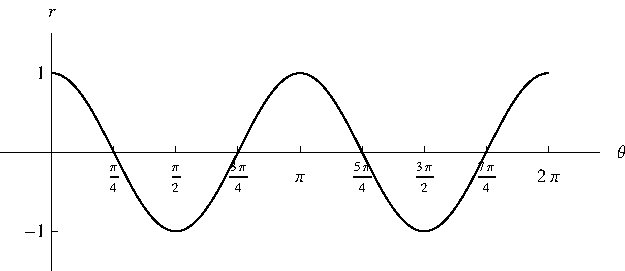
\includegraphics[height=3.6cm]{polar-curves/pictures/11-03-ex8helpera.pdf}%
%}%
%\only<handout:0| 2>{%
%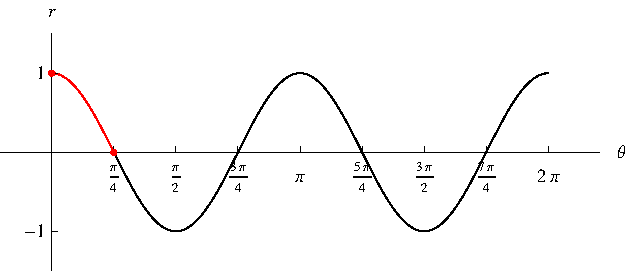
\includegraphics[height=3.6cm]{polar-curves/pictures/11-03-ex8helperb.pdf}%
%}%
%\only<handout:0| 3>{%
%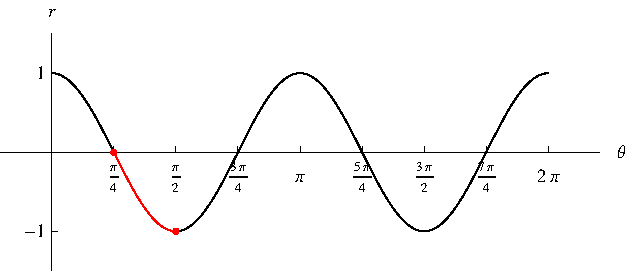
\includegraphics[height=3.6cm]{polar-curves/pictures/11-03-ex8helperc.pdf}%
%}%
%\only<handout:0| 4>{%
%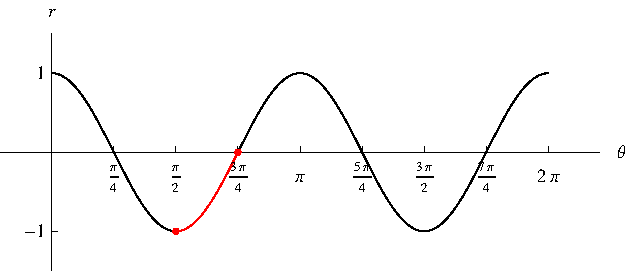
\includegraphics[height=3.6cm]{polar-curves/pictures/11-03-ex8helperd.pdf}%
%}%
%\only<handout:0| 5>{%
%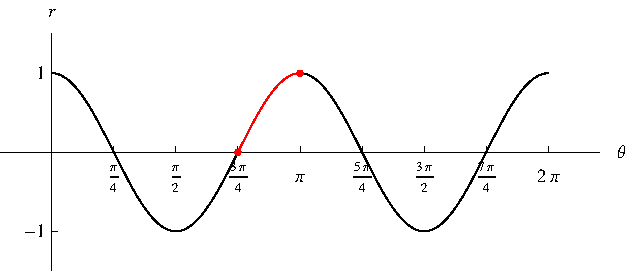
\includegraphics[height=3.6cm]{polar-curves/pictures/11-03-ex8helpere.pdf}%
%}%
%\only<handout:0| 6>{%
%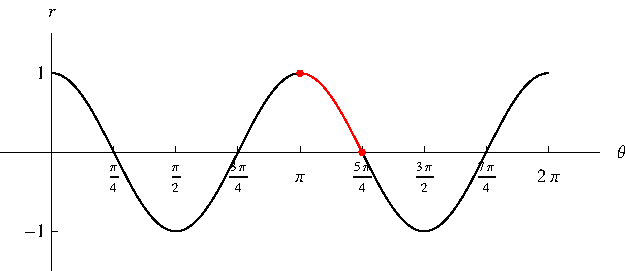
\includegraphics[height=3.6cm]{polar-curves/pictures/11-03-ex8helperf.pdf}%
%}%
%\only<handout:0| 7>{%
%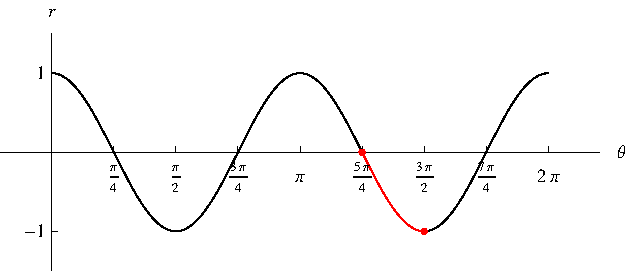
\includegraphics[height=3.6cm]{polar-curves/pictures/11-03-ex8helperg.pdf}%
%}%
%\only<handout:0| 8>{%
%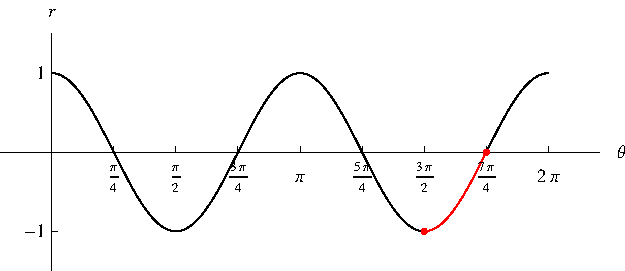
\includegraphics[height=3.6cm]{polar-curves/pictures/11-03-ex8helperh.pdf}%
%}%
%\only<9->{%
%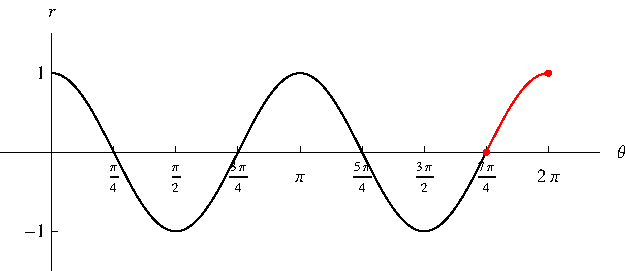
\includegraphics[height=3.6cm]{polar-curves/pictures/11-03-ex8helperi.pdf}%
%}%
\end{columns}
\end{example}
\end{frame}
% end module polar-curve-ex8
